\documentclass{beamer}
\beamertemplatenavigationsymbolsempty
\usepackage[french]{babel}
\usepackage{fontspec}
\usepackage{amsmath, amsthm, amsfonts}
\usepackage[separate-uncertainty]{siunitx}
\usepackage{xcolor}
\usepackage{tikz}
\usepackage{tikz-cd}
\usepackage[object=vectorian]{pgfornament}
\usepackage{circuitikz}
\usepackage{hyperref}
\usepackage{caption}
\usepackage{booktabs}
\usepackage{mathtools}
\usepackage{longtable}
\usepackage[version=3]{mhchem}
\usepackage{marginnote}
\usepackage[framemethod=tikz]{mdframed}


% Paul Tol's qualitative palette
% ``bright''.https://personal.sron.nl/~pault/#sec:qualitative
\definecolor{tblue}{HTML}{4477AA}
\definecolor{tcyan}{HTML}{66CCEE}
\definecolor{tgreen}{HTML}{228833}
\definecolor{tyellow}{HTML}{CCBB44}
\definecolor{tred}{HTML}{EE6677}
\definecolor{tpurple}{HTML}{AA3377}
\definecolor{tgrey}{HTML}{BBBBBB}


% Justification for marginnotes.
\renewcommand*{\raggedleftmarginnote}{}
\renewcommand*{\raggedrightmarginnote}{}


% Styles for mdframed environments.
\newmdenv[backgroundcolor=tgreen!10,linecolor=tgreen!30]{reponsebox}
\newmdenv[backgroundcolor=tyellow!10,linecolor=tyellow!30]{diapobox}
\newmdenv[backgroundcolor=tred!10,linecolor=tred!30]{fondamentalbox}

% Default arrow for tikz and style for positive and negative objects.
\tikzset{>=latex,
    negative/.style={draw=teal!70!black, fill=teal!10, thick},
    positive/.style={draw=red, fill=red!10, thick}}
\usetikzlibrary{matrix,calc,decorations.pathreplacing,decorations.pathmorphing,decorations.markings}

% French locale for numbers and negative exponent for units.
\sisetup{locale=FR, per-mode=symbol}

\newcommand{\abs}[1]{\left| #1 \right|}
\newcommand{\rhat}{\vec{\hat{r}}}
\newcommand{\xhat}{\vec{\imath}}
\newcommand{\yhat}{\vec{\jmath}}
\newcommand{\zhat}{\vec{k}}
\newcommand{\real}{\mathbb{R}}
\newcommand{\der}[2]{\frac{\mathrm{d}#1}{\mathrm{d}#2}}
\newcommand{\pder}[2]{\frac{\partial\ #1}{\partial\ #2}}
\newcommand{\dif}{\mathrm{d}}
\newcommand{\ddif}{\,\mathrm{d}}
\newcommand{\grad}{\vec{\nabla}}
\newcommand{\exemple}[1]{\begin{fullwidth}#1\end{fullwidth}}
\newcommand{\norm}[1]{\lVert\ #1\ \rVert}
\newcommand{\vu}{\vec{u}}
\newcommand{\vv}{\vec{v}}
\newcommand{\vr}{\vec{r}}
\newcommand{\va}{\vec{a}}
\newcommand{\vF}{\vec{F}}
\newcommand{\vE}{\vec{E}}
\newcommand{\vB}{\vec{B}}
\newcommand{\vecxyz}[3]{#1 \xhat\ + #2 \yhat\ + #3 \zhat}
\newcommand{\vecxy}[2]{#1 \xhat\ + #2 \yhat}
\newcommand{\coulombcst}{k}
\newcommand{\emf}{\ensuremath{\mathcal{E}}}
\newcommand{\eval}{\SI{1.602e-19}{C}}
\newcommand{\kval}{\SI{8.99e9}{Nm^2 \per C^2}}

% Nice separator line
\newcommand{\sectionline}{
    \noindent
    \begin{center}
        \resizebox{0.5\linewidth}{1ex}
    {{%
    {\begin{tikzpicture}
    \node  (C) at (0,0) {};
    \node (D) at (9,0) {};
    \path (C) to [ornament=85] (D);
    \end{tikzpicture}}}}
    \end{center}
}

\theoremstyle{definition}
\newtheorem*{defn}{Definition}


\usepackage[version=3]{mhchem}

\setbeamercolor{title}{fg=tblue}
\setbeamercolor{frametitle}{fg=tblue}
\setbeamercolor{structure}{fg=tblue}

% Make footnotesize smaller
\makeatletter
\renewcommand\footnotesize{%
   \@setfontsize\footnotesize\@viipt{11}%
   \abovedisplayskip 8\p@ \@plus2\p@ \@minus4\p@
   \abovedisplayshortskip \z@ \@plus\p@
   \belowdisplayshortskip 4\p@ \@plus2\p@ \@minus2\p@
   \def\@listi{\leftmargin\leftmargini
               \topsep 4\p@ \@plus2\p@ \@minus2\p@
               \parsep 2\p@ \@plus\p@ \@minus\p@
               \itemsep \parsep}%
   \belowdisplayskip \abovedisplayskip
}
\makeatother

\title{Électricité et magnétisme}
\subtitle{Chapitre 8 - Champ magnétique}
\date{10 novembre 2021}
\author{Loïc Séguin-Charbonneau}
\institute{Cégep Édouard-Montpetit}

\begin{document}

\maketitle

\begin{frame}[t]{Exercice sur les aimants}

  Déterminer si les deux objets s'attirent, se repoussent, ou n'exercent aucune
  force l'un sur l'autre. (Note: les lignes de champ ne sont tracées que
  partiellement.)

  \begin{center}
    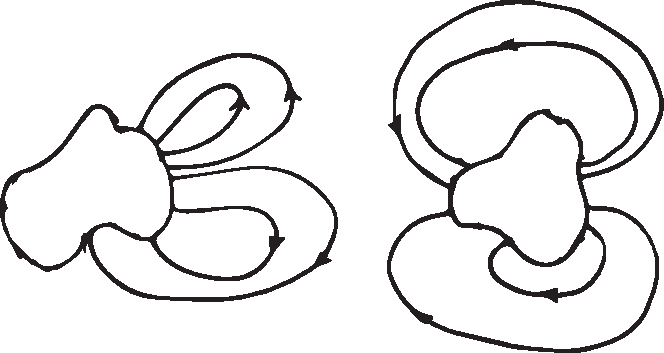
\includegraphics[scale=0.6]{figures/exercice-champ-magnetique1a.pdf}
  \end{center}

  \begin{enumerate}[A.]
    \item S'attirent
    \item Se repousent
    \item N'exercent aucune force l'un sur l'autre
  \end{enumerate}

\end{frame}


\begin{frame}[t]{Exercice sur les aimants}

  Déterminer si les deux objets s'attirent, se repoussent, ou n'exercent aucune
  force l'un sur l'autre. (Note: les lignes de champ ne sont tracées que
  partiellement.)

  \begin{center}
    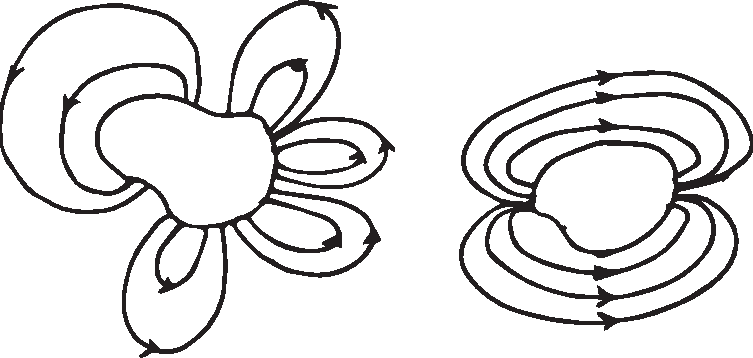
\includegraphics[scale=0.6]{figures/exercice-champ-magnetique1b.pdf}
  \end{center}

  \begin{enumerate}[A.]
    \item S'attirent
    \item Se repousent
    \item N'exercent aucune force l'un sur l'autre
  \end{enumerate}

\end{frame}


\begin{frame}[t]{Exercice sur les aimants}
  
  Déterminer si les deux objets s'attirent, se repoussent, ou n'exercent aucune
  force l'un sur l'autre. (Note: les lignes de champ ne sont tracées que
  partiellement.)

  \begin{center}
    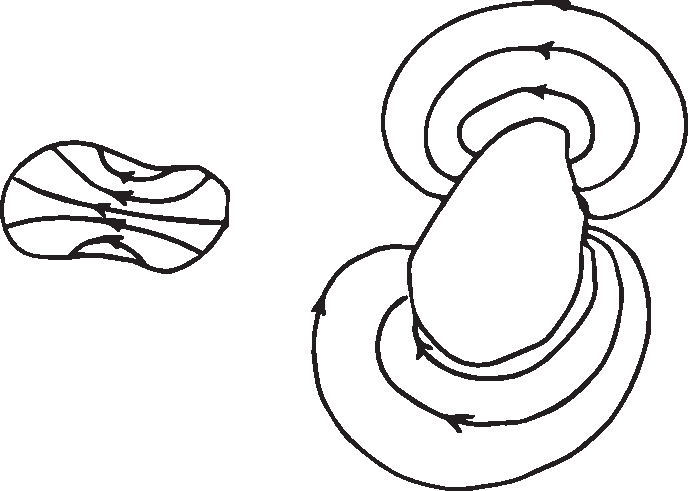
\includegraphics[scale=0.6]{figures/exercice-champ-magnetique1c.pdf}
  \end{center}

  \begin{enumerate}[A.]
    \item S'attirent
    \item Se repousent
    \item N'exercent aucune force l'un sur l'autre
  \end{enumerate}

\end{frame}


\begin{frame}[t]{Exercice sur les aimants}

  Déterminer si les deux objets s'attirent, se repoussent, ou n'exercent aucune
  force l'un sur l'autre. (Note: les lignes de champ ne sont tracées que
  partiellement.)

  \begin{center}
    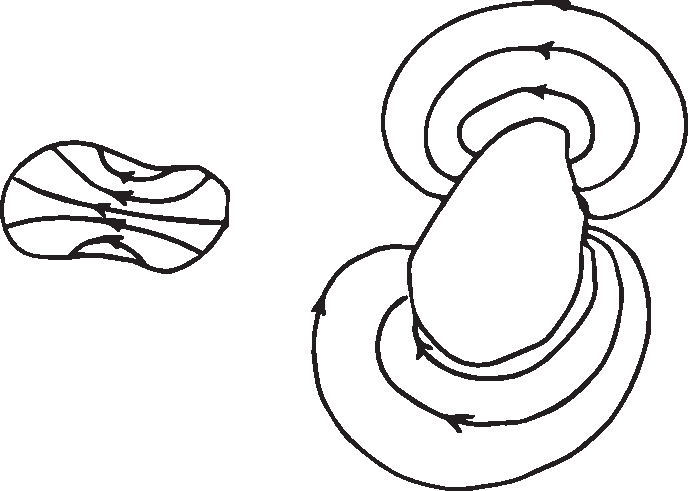
\includegraphics[scale=0.6]{figures/exercice-champ-magnetique1c.pdf}
  \end{center}

  \begin{enumerate}[A.]
    \item S'attirent
    \item Se repousent
    \item N'exercent aucune force l'un sur l'autre
  \end{enumerate}

\end{frame}


\begin{frame}[t]{Champ magnétique d'un fil}
  
  Quelle image illustre correctement le champ magnétique produit par le courant
  dans le fil?

  \begin{center}
    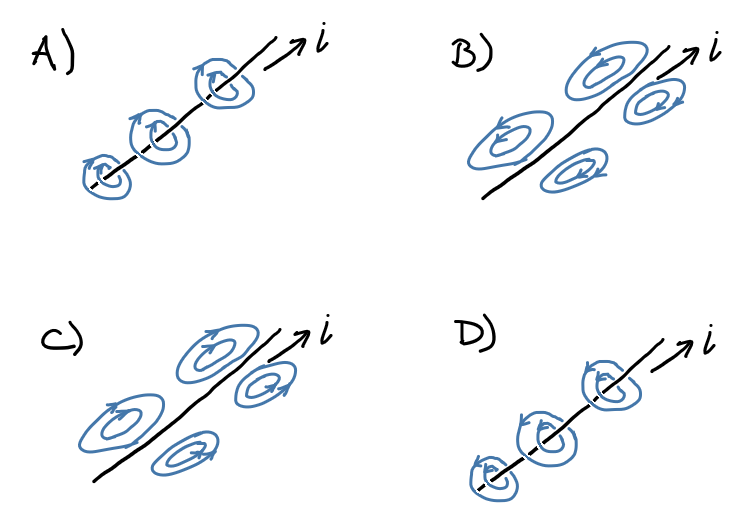
\includegraphics[scale=0.5]{figures/champ_fil_ex1.png}
  \end{center}

\end{frame}


\begin{frame}[t]{Champ magnétique d'un fil}
  
  Quelle image illustre correctement le champ magnétique produit par le courant
  dans le fil?

  \begin{center}
    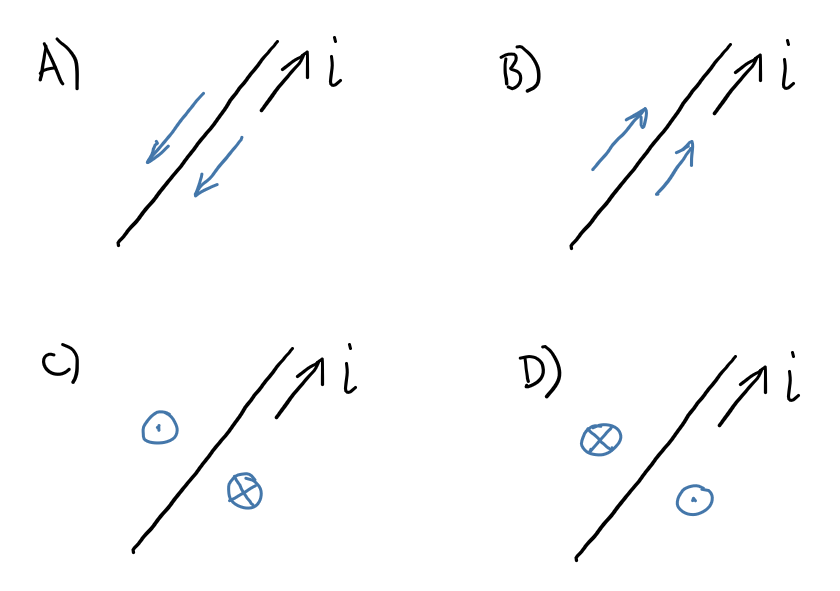
\includegraphics[scale=0.4]{figures/champ_fil_ex2.png}
  \end{center}

\end{frame}


\begin{frame}[t]{Champ magnétique d'une boucle}
  
  Quelle image illustre correctement le champ magnétique produit par le courant
  dans la boucle?

  \begin{center}
    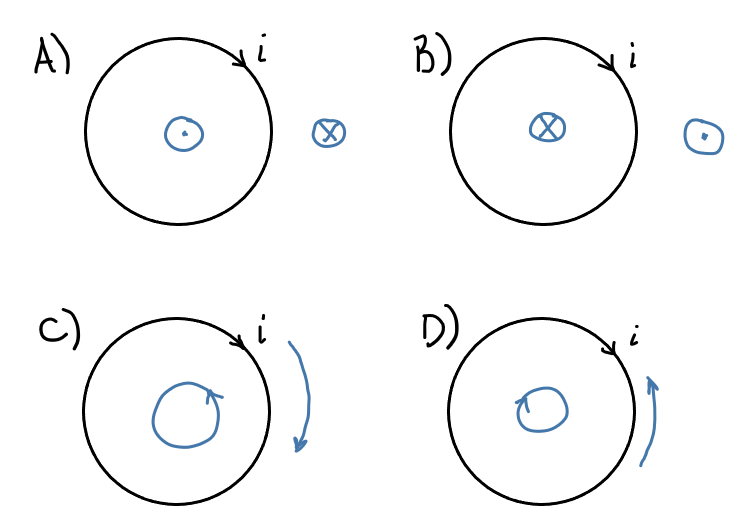
\includegraphics[scale=0.4]{figures/champ_boucle_ex1.png}
  \end{center}

\end{frame}


\begin{frame}[t]{Champ magnétique d'une boucle}
  
  Quelle image illustre correctement le champ magnétique produit par le courant
  dans la boucle?

  \begin{center}
    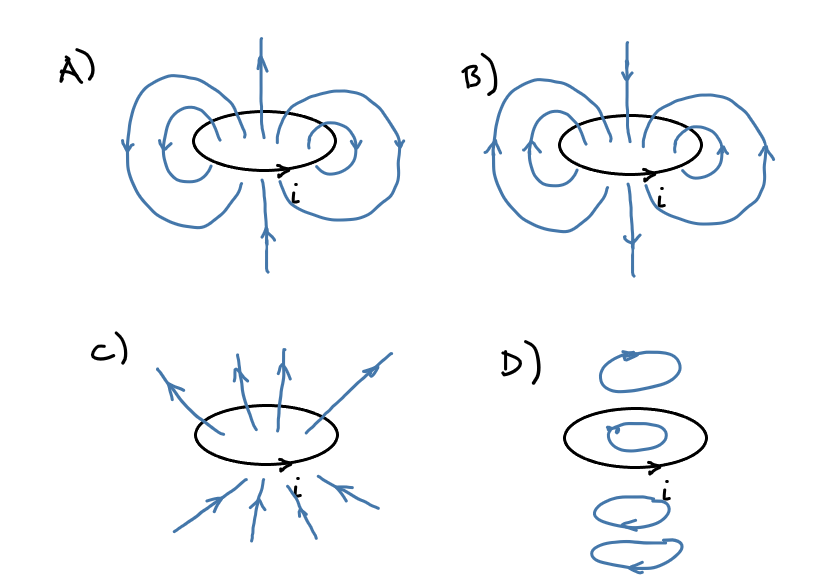
\includegraphics[scale=0.4]{figures/champ_boucle_ex2.png}
  \end{center}

\end{frame}


\begin{frame}[t]{Champ magnétique d'un aimant}
  
  Quelle image illustre correctement les petites boucles de courant qui
  génèrent le champ d'un aimant?

  \begin{center}
    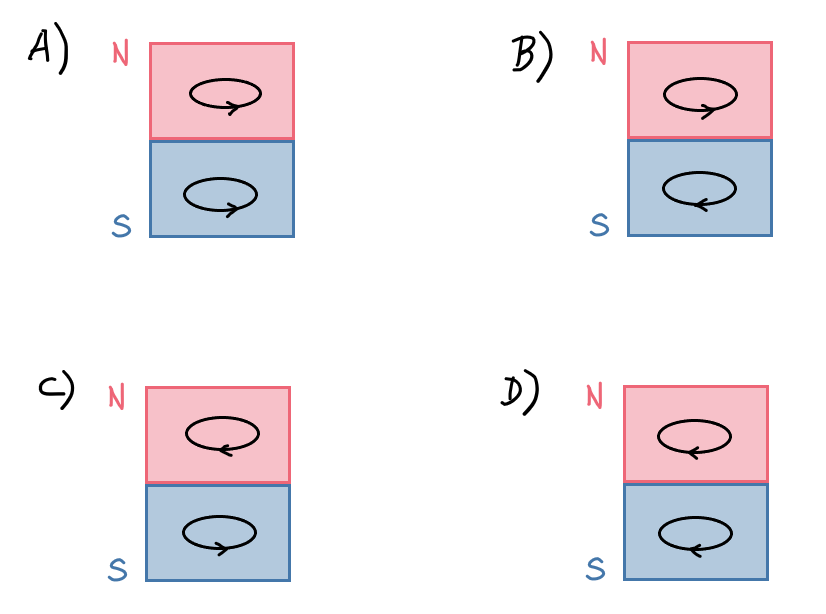
\includegraphics[scale=0.4]{figures/aimant_boucle.png}
  \end{center}

\end{frame}


\begin{frame}{Produit vectoriel}
  Classer les situations suivantes en ordre croissant de la grandeur du produit
  $\abs{\vu \times \vv}$.

  \begin{center}
    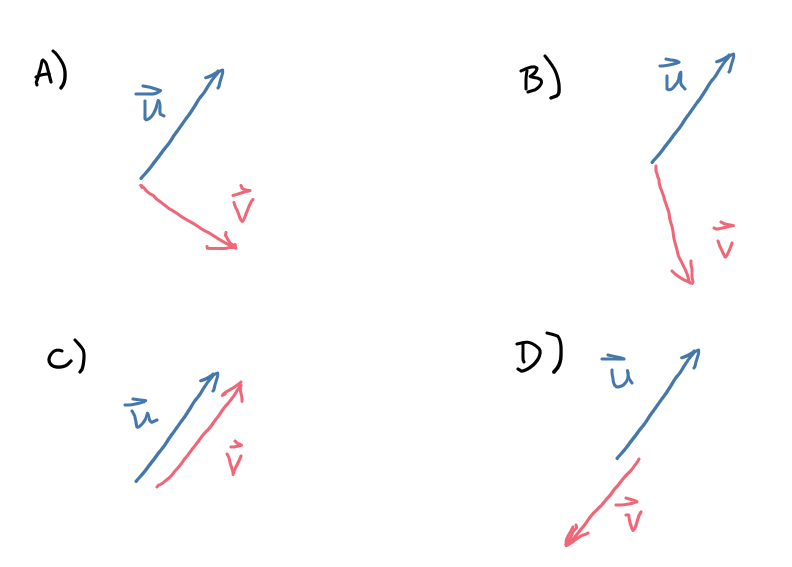
\includegraphics[scale=0.5]{figures/produit-vec_ex1.png}
  \end{center}
\end{frame}


\begin{frame}{Produit vectoriel}
  Calculer le produit vectoriel du vecteur $\vu = \vecxyz{3}{-2}{1}$ et du
  vecteur $\vv$ dans le plan $xy$, de longueur $2$ et qui fait un angle de
  \SI{30}{\degree} avec l'axe des $x$ positifs.
\end{frame}


\begin{frame}[t]{Imagerie par résonance magnétique}
  \begin{columns}
    \column{0.5\textwidth}

    \begin{center}
      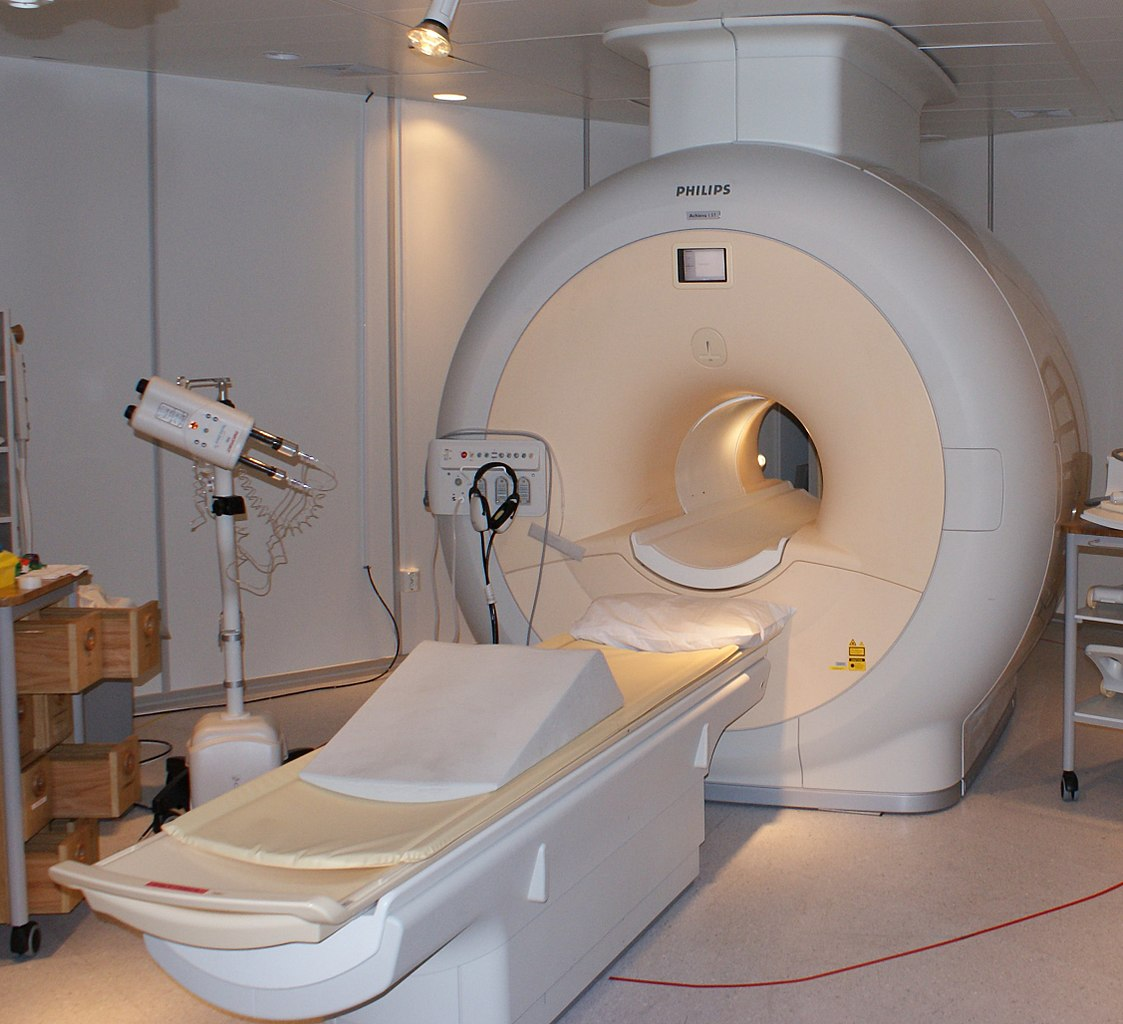
\includegraphics[width=\textwidth]{figures/MRI-Philips.jpg}
    \end{center}

    \column{0.5\textwidth}

    \begin{center}
      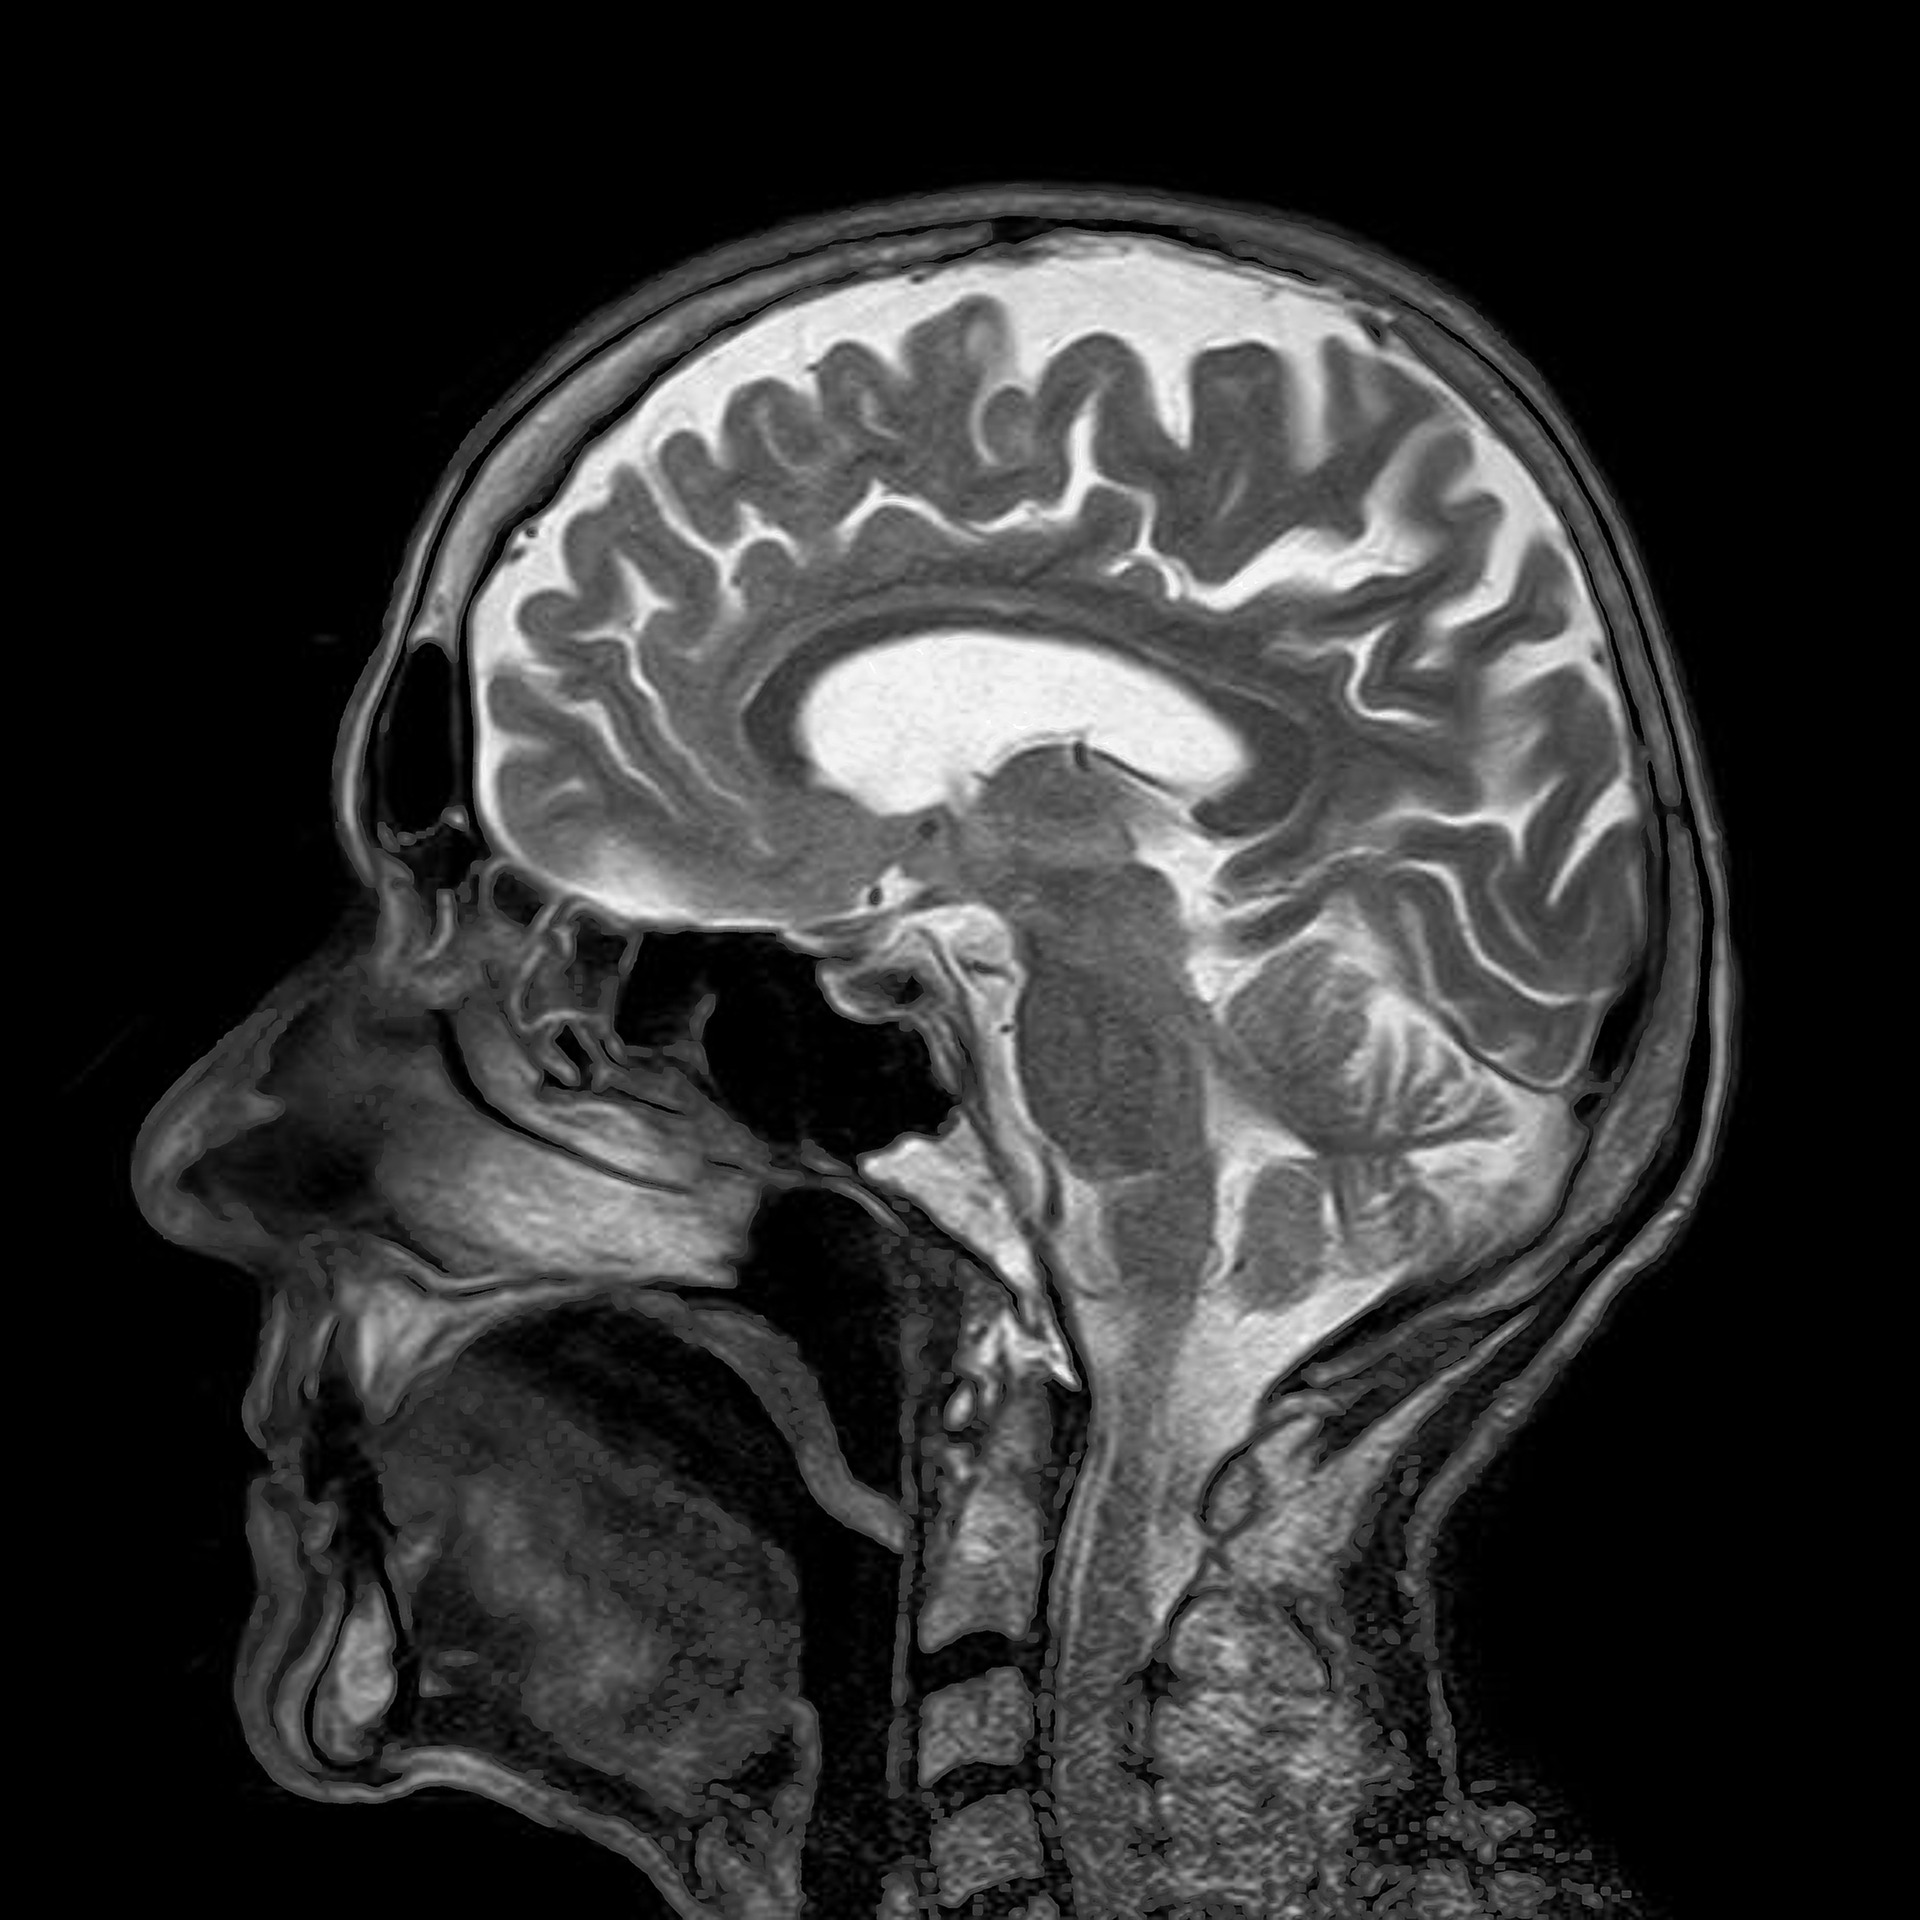
\includegraphics[width=\textwidth]{figures/mri-brain.jpg}
    \end{center}
  \end{columns}
\end{frame}


\begin{frame}[t]{Imagerie par résonance magnétique}
  Une machine typique produit un champ magnétique de \SI{1.50}{\tesla} au
  centre d'une bobine faite d'un supraconducteur. Si la bobine est faite de
  \num{10000} tours de fil et a un rayon de $R = \SI{50}{\centi\meter}$, quel
  est le courant qui doit circuler dans le fil?

  \only<2>{
    Quelle figure illustre correctement la situation?
    \begin{center}
      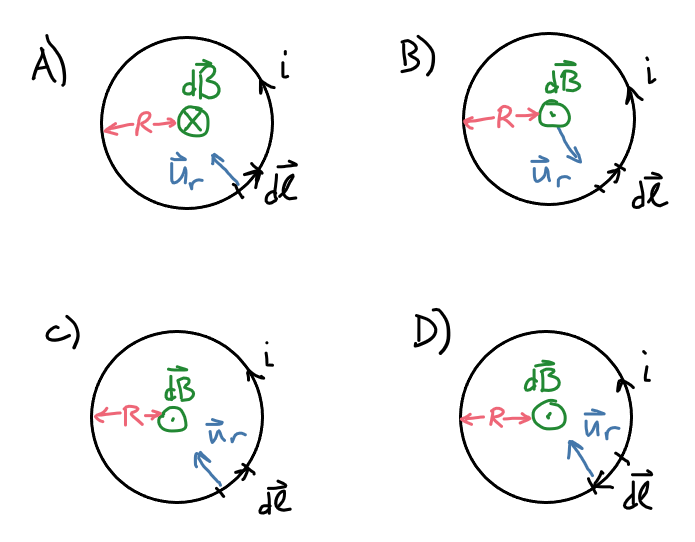
\includegraphics[scale=0.4]{figures/mri_draw.png}
    \end{center}
  }
  \only<3-4>{
    Dans la loi de Biot-Savart
    $$d\vB = \frac{\mu_0 i}{4\pi r^2} d\vec{\ell} \times \vu_r$$
    que vaut $r$?

    \begin{enumerate}[A.]
      \item \SI{100}{\centi\meter}
      \item<alert@4> \SI{50}{\centi\meter}
      \item \SI{-50}{\centi\meter}
      \item Ça dépend du bout de fil qu'on considère
    \end{enumerate}
  }
  \only<5-6>{
    Dans la loi de Biot-Savart
    \begin{columns}
      \column{0.5\textwidth}
      $$d\vB = \frac{\mu_0 i}{4\pi r^2} d\vec{\ell} \times \vu_r$$
      \column{0.5\textwidth}
      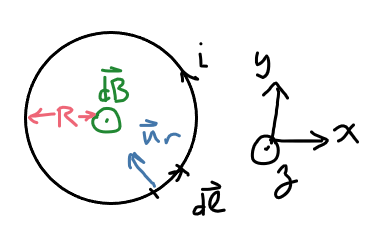
\includegraphics[scale=0.4]{figures/mri_figure_correcte.png}
    \end{columns}
    que vaut $d\vec{\ell} \times \vu_r$?

    \begin{enumerate}[A.]
      \item $d\vec{\ell}$
      \item<alert@6> $d\ell\, \zhat$
      \item $-d\ell\, \zhat$
      \item $\vec{0}$
    \end{enumerate}
  }
  \only<7-8>{
    Quelle est la forme simplifiée de la loi de Biot-Savart dans ce contexte?
    \begin{columns}
      \column{0.5\textwidth}
      $$d\vB = \frac{\mu_0 i}{4\pi r^2} d\vec{\ell} \times \vu_r$$
      \column{0.5\textwidth}
      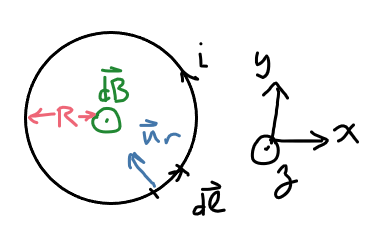
\includegraphics[scale=0.3]{figures/mri_figure_correcte.png}
    \end{columns}

    \begin{enumerate}[A.]
      \item $\displaystyle{
          d\vB = \frac{\mu_0 i}{4\pi R^2} d\vec{\ell} \cos \SI{90}{\degree}}$
      \item $\displaystyle{
          d\vB = \frac{\mu_0 i}{4\pi r^2} d\ell \sin \SI{90}{\degree}}$
      \item $\displaystyle{
          d\vB = -\frac{\mu_0 i \zhat}{4\pi r^2} d\ell}$
      \item<alert@8> $\displaystyle{
          d\vB = \frac{\mu_0 i \zhat}{4\pi R^2} d\ell}$
    \end{enumerate}
  }
  \only<9-10>{
    On applique le principe de superposition pour trouver le champ total
    $$\vB = \int_\mathrm{boucle} \frac{\mu_0 i}{4\pi r^2} d\vec{\ell} \times \vu_r$$
    Quel est le résultat?

    \begin{enumerate}[A.]
      \item $\displaystyle{\vB = \frac{\mu_0 i}{4\pi R^2}}$
      \item $\displaystyle{\vB = \frac{\mu_0 i}{4\pi R^2} \zhat}$
      \item $\displaystyle{\vB = \frac{\mu_0 i}{4\pi R} \zhat}$
      \item<alert@10> $\displaystyle{\vB = \frac{\mu_0 i}{2R} \zhat}$
    \end{enumerate}
  }
  \only<11-12>{
    Comment fait-on pour tenir compte du fait qu'il y a \num{10000} tours de
    fil?

    \begin{enumerate}[A.]
      \item Ça ne change rien au résultat qu'on a obtenu.
      \item<alert@12> Chaque boucle génère un champ magnétique de
        $\SI{1.50}{\tesla}/\num{10000}$
        donc on utilise cette valeur pour $B$.
      \item<alert@12> Le courant total produit par la bobine est \num{10000} fois le
        courant dans un seul fil, donc on multiplie l'expression de droite par
        \num{10000}.
      \item C'est comme si le rayon de la bobine était \num{10000} fois plus
        grand, on multiplie donc la valeur de $R$ par \num{10000}.
    \end{enumerate}
  }

\end{frame}


\begin{frame}{Réacteur ITER}
  \begin{columns}
    \column{0.4\textwidth}
    \begin{center}
      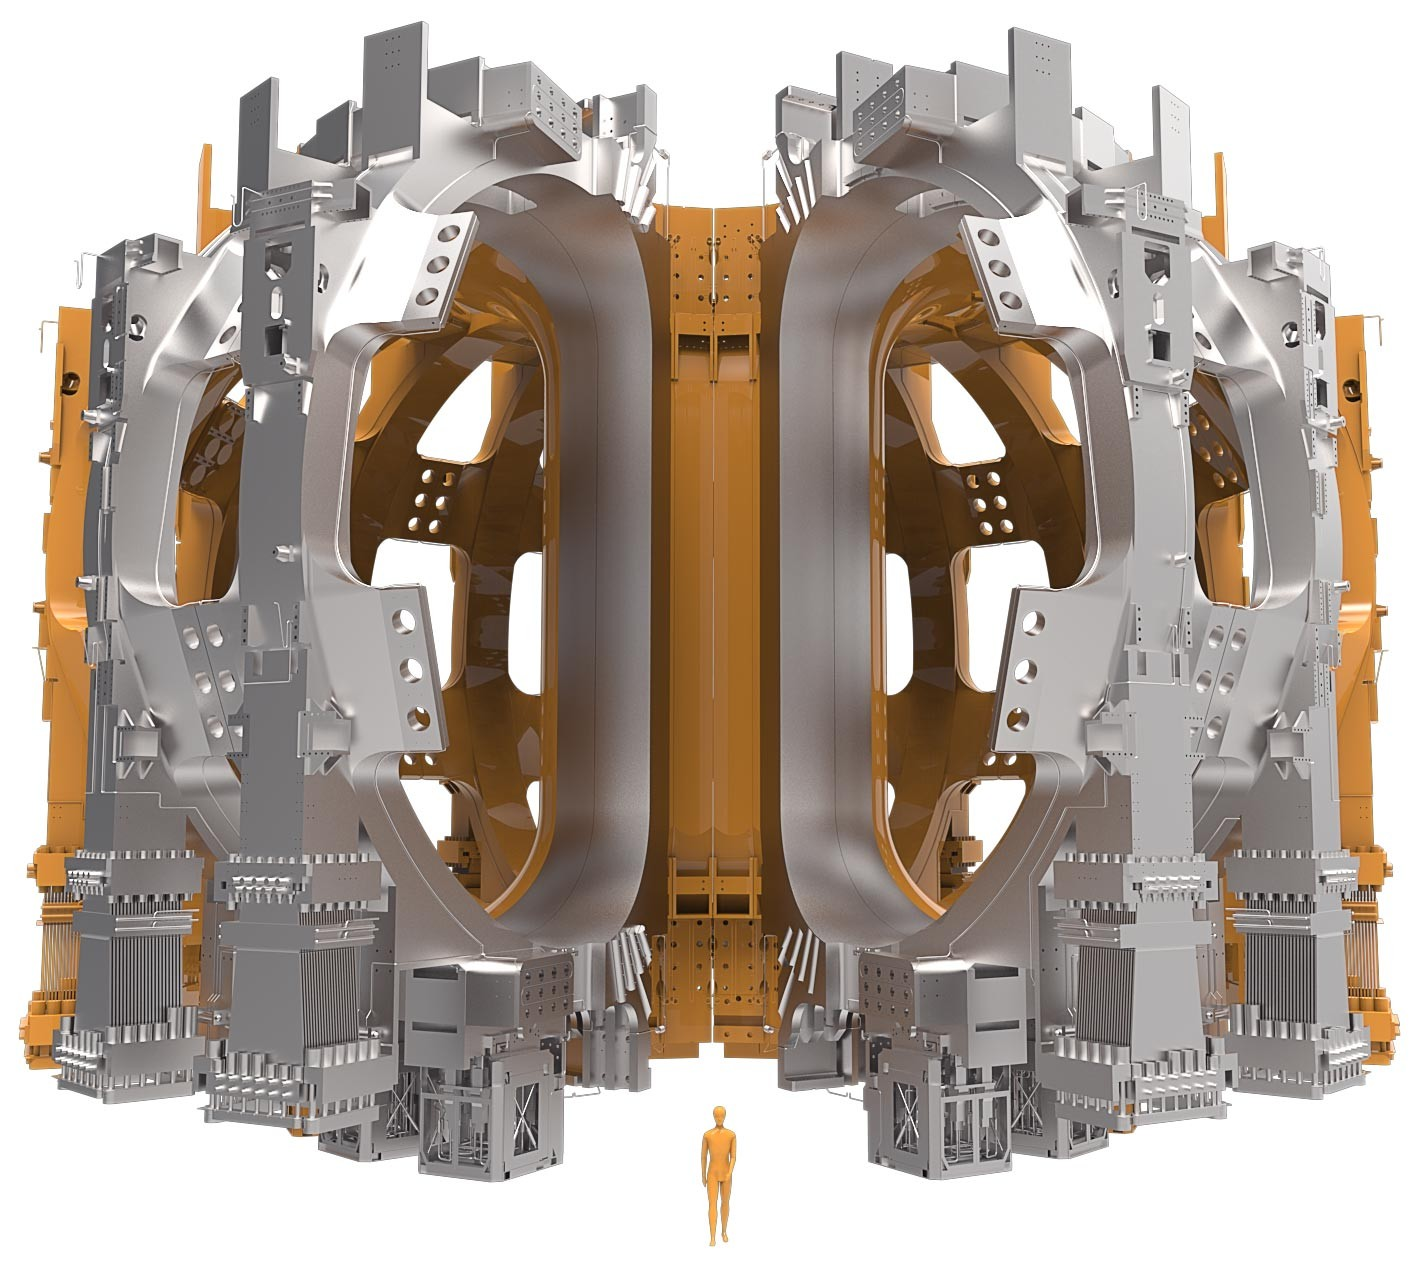
\includegraphics[width=\textwidth]{figures/iter_toroidal_coil.jpg}
    \end{center}
    \column{0.6\textwidth}
    \begin{center}
      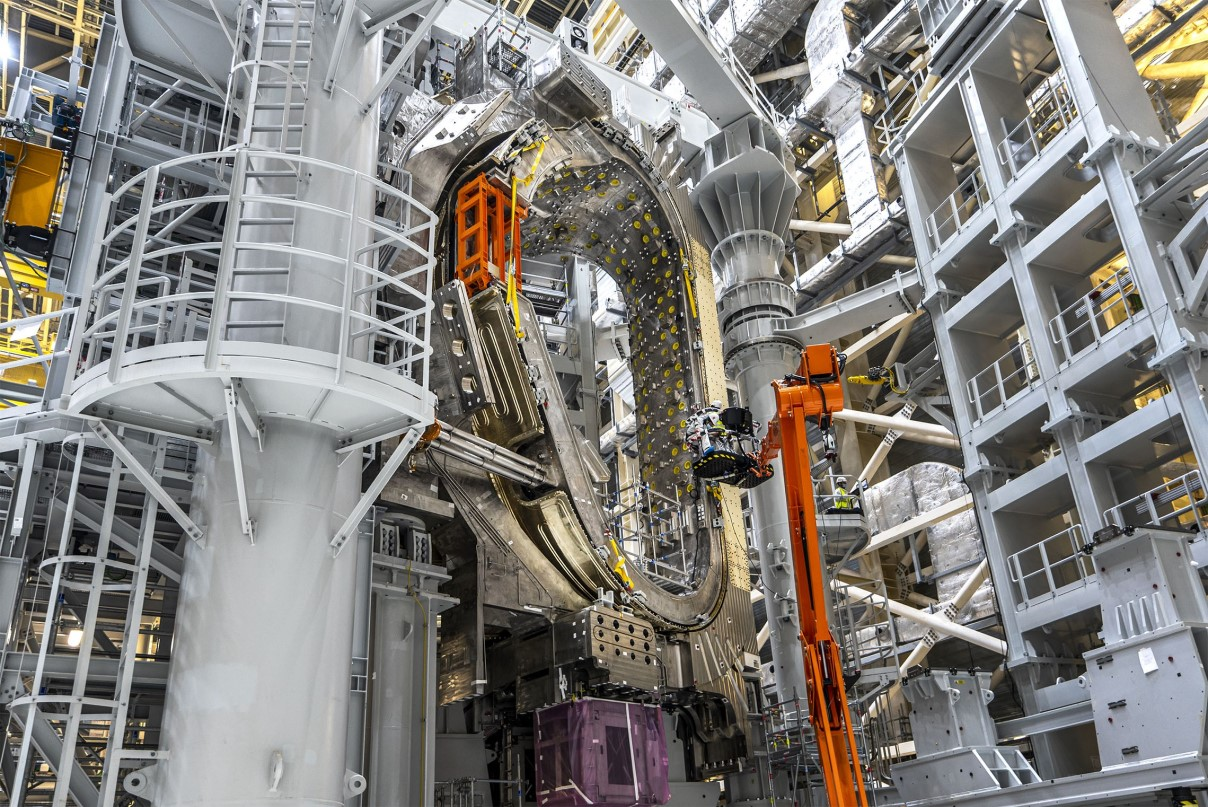
\includegraphics[width=\textwidth]{figures/sector_6_sub_assembly_3_small.jpg}
    \end{center}
  \end{columns}
\end{frame}


\begin{frame}{Réacteur ITER}
  Le réacteur à fusion nucléaire ITER est constitué d'une cavité toroïdale dans
  laquelle un plasma à haute température est confiné grâce à un champ
  magnétique de \SI{5.3}{\tesla}. Le champ magnétique est produit par un
  solénoïde toroïdal (un solénoïde dont les extrémités sont reliées ensembles).
  Le tore a un rayon d'environ \SI{6.2}{\meter} et les spires ont un rayon
  d'environ \SI{6.5}{\meter}. Le courant qui circule dans le câble est de
  \SI{68}{\kilo\ampere}. Quelle est la longueur de câble totale utilisée dans
  le solénoïde?

  \begin{center}
    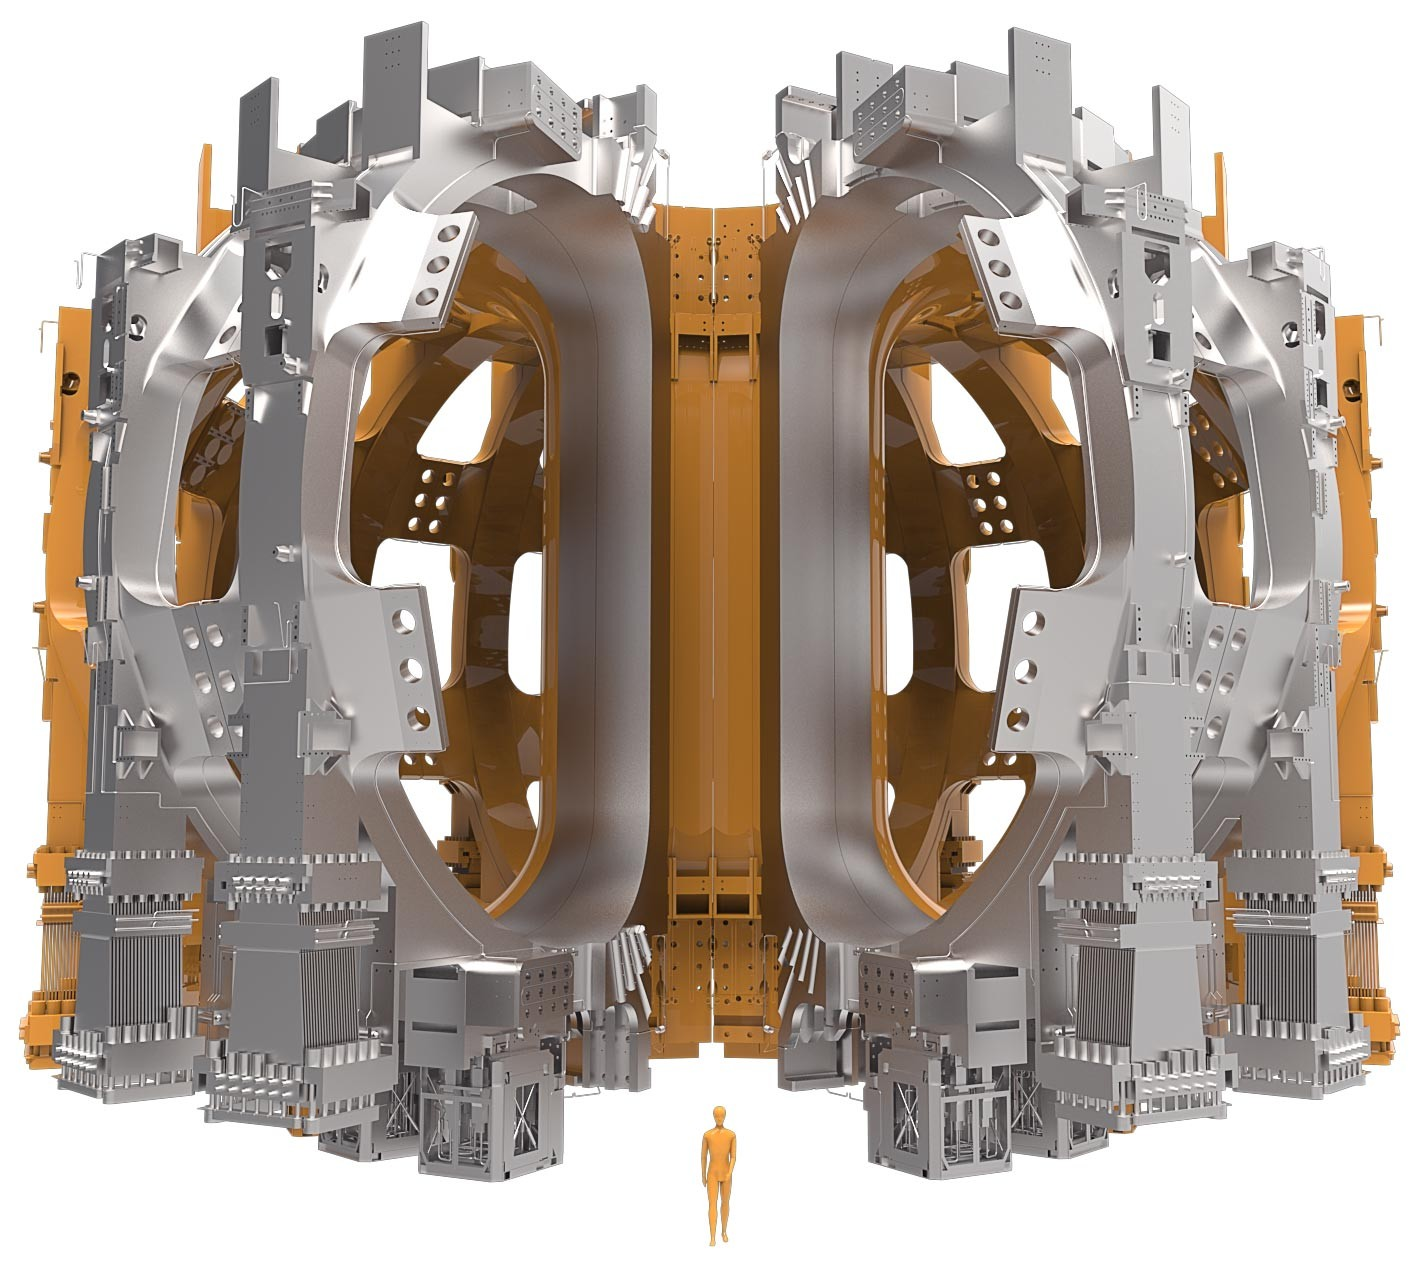
\includegraphics[width=0.5\textwidth]{figures/iter_toroidal_coil.jpg}
  \end{center}
\end{frame}

\end{document}
